\section{Admin-Client HomeScreen}

Über den Home-Screen des Admin-Clients kann per Druck eines Buttons der Scan-Vorgang
von QR-Codes gestartet werden. Dabei wechselt die App zur Frontkamera des Gerätes und startet den Scanner.

\subsection{Scannen von QR-Codes}

Für das reibungslose Einscannen eines QR-Codes wird das \textit{flutter\_barcode\_scanner}-Package
verwendet.\cite{flutterBarcodeScanner2021}

Mithilfe dieses Packages kann dynamisch ein neues View mit der Frontkamera, mit welcher auch 
ein QR-Code eingescanned wird, geöffnet werden.\\
Dies geschieht auf folgende Weise:

\begin{code}[H]
    \centering
    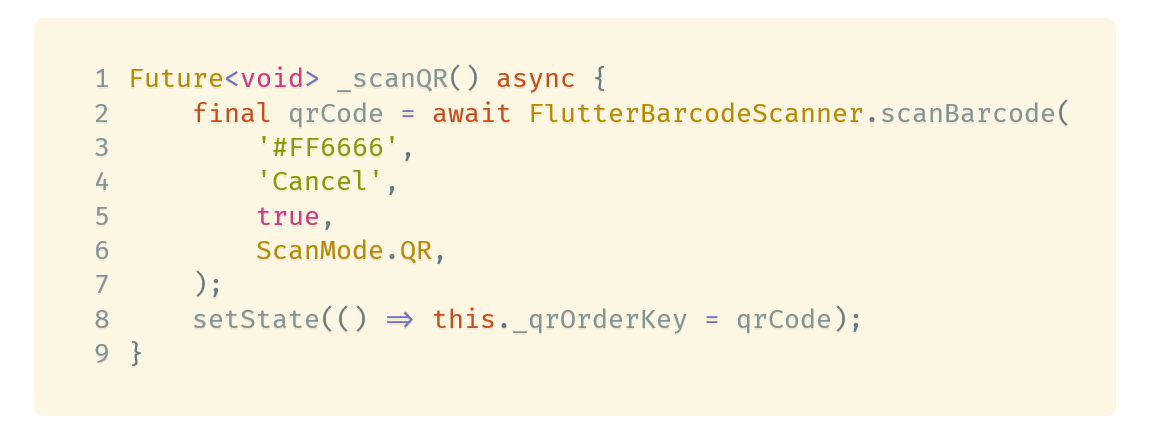
\includegraphics[width=1\textwidth]{images/Admin-Client/screens/scanQR.png}
    \vspace{-25pt}
    \caption{Öffnen des QR-Scanners}
\end{code}

Wird nun obige Funktion mittels Antippen des Buttons im Screen ausgeführt, öffnet sich die 
Kamera-App des Geräts und beginnt mit dem Scanvorgang, so muss der Fokus nur noch auf einen 
QR-Code gerichtet werden.

\begin{figure}[H]
    \centering
    \hfill
    \subfigure[Home-Screen des Admin-Clients mit Scan-Button]{
\includegraphics[width=0.4\textwidth]{images/Admin-Client/screens/homescreen.png}}
    \hfill
    \subfigure[QR-Code-Scanner des Admin-Clients]{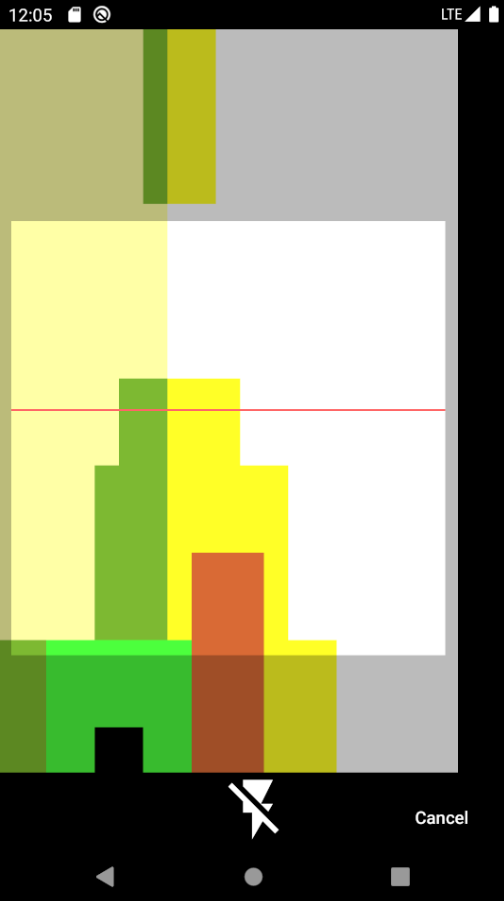
\includegraphics[width=0.40\textwidth]{images/Admin-Client/screens/QRScanner.png}}
    \hfill
    \caption{Wechsel von Home-Screen zum QR-Code-Scanner}
\end{figure}

Nach einem erfolgreichen Scan-Vorgang wird automatisch ein Request an die API gesendet und die
Gültigkeit des QR-Codes überprüft.

Stellt sich dabei heraus, dass der Code aus folgenden Gründen

\begin{itemize}
    \item Bestellung wurde nicht am Vortag aufgegeben
    \item Order-ID und User-ID passen nicht zusammen
    \item Bestellung wurde bereits invalidiert
\end{itemize}

nicht gültig ist, wird über einen Alert-Dialog eine entsprechende Fehlermeldung im Admin-Client
angezeigt.

Wenn der Code als valide gilt wird ein Alert-Dialog geöffnet, in dem alle relevanten Informationen
der Bestellung wie bestellte Waren und deren Preis aufgelistet.\\
Über dieses Dialogfenster lässt sich in weiterer Folge die Bestellung per Button-Druck, der einen
Invalidierungs-Request an die API auslöst, ungültig machen und damit als abgeschlossen markieren.